\documentclass[11pt,a4paper]{article}
\usepackage[margin=2.2cm]{geometry}
\usepackage[T1]{fontenc}\usepackage{lmodern,microtype}
\usepackage{amsmath,booktabs,graphicx,xurl}
\usepackage[numbers,sort&compress]{natbib}\usepackage[hidelinks]{hyperref}
\usepackage{placeins}
\setlength{\parindent}{0pt}\setlength{\parskip}{0.35em}
\setlength{\emergencystretch}{2em}
\title{Fresh-seed mechanism replication\\\large Results, eligibility and discussion}
\author{Effectome-to-behavior project}\date{17 November 2026}
\begin{document}\maketitle
\section{Completed study and interpretation boundary}
All 119 declared cells completed, with 714 available method/control
entries. This study evaluates the revised outgoing-disconnection readout in the
fully observed, model-matched control. It does not replace the old 560-run
latent-bistable benchmark, validate a learned behavioral manifold, or include
graph-similarity experiments. The imported native estimators remain c-GC/c-GC*
and fastC-GC/fastC-GC* \citep{adedayo2025cgc,adedayo2026fastcgc}.

The paired native comparisons show 97.55--98.36\% lower mean effect MAE at the
longer history across 20 fresh process seeds. Exact null outcomes and the
individual-ranking eligibility limit are reported separately below. These provide
positive evidence for effect estimation within this control while preserving the
original acceptance decision.

The frozen all-four bounded-control acceptance flag is \textbf{False}.
Complete execution, accurate effect estimation, applicable individual-neuron
ranking and null specificity are different outcomes. Ineligible evidence is
retained, not silently dropped to obtain a passing decision.

\section{Frozen design and calibration}
The primary discovery history is 1,024 samples; a 256-sample history is paired on
the same positive-test recordings. Each seed has 24 trials of length 1,152 and six
observed neurons. Twelve trials supply mechanism fitting, including three reserved
for penalty/noise selection; native discovery sees only the nine inner-training
trials. Twelve whole trials are held out. This ownership prevents evaluation from
selecting fit parameters \citep{cawley2010overfitting}. Known support supplies only
adjacency to its explicit oracle lane; native lanes learn support and all lanes
fit coefficients/noise. Ridge fitting uses the declared additive-tanh basis
\citep{hoerl1970ridge,peters2014additive}; this favorable match does not establish
general causal identifiability.

The disjoint pools contain 19 calibration-null seeds, 20 positive-test
seeds and 60 null-test seeds. For each method, one calibration score is the
maximum estimated probability effect across eight candidates and both directions
within a seed. Its rank is $r=\lceil(n+1)(1-0.05)\rceil$. The operational cutoff
is the larger of that ordered calibration score and the existing 0.10 minimum
effect size, with strict exceedance for nomination. Thresholds were locked before
test jobs were submitted. The finite-sample rank principle gives marginal global-null
protection under exchangeability \citep{angelopoulos2021conformal}; it does not
certify a realized cutoff's conditional false-event rate at 95\% confidence.

Conventional CPU permutation randomness is not controlled by the public seed API
in the pinned upstream package. Its randomization is part of the fixed scoring
procedure. First-completed native evidence is retained, and favorable reruns are
not selected. Exchangeability of randomized scores is an assumption, not a claim
of controlled or byte-identical conventional random streams.

\section{Effect estimation and individual ranking}
Effect MAE compares estimated with simulator probability reductions after outgoing
disconnection. This structural operation differs from refitting a predictive
model without graph features \citep{pearl2010causalinference,williamson2023importance}.
Brier scores concern observed factual binary events. Top-k and nomination recall
concern intervention-positive neurons; nomination precision includes all declared
candidate units/groups. Table~\ref{tab:primary} preserves the planned denominators.

\begin{table}[htbp]\centering\scriptsize\setlength{\tabcolsep}{3.5pt}
\caption{Primary history. MAE and Brier use the complete planned positive-seed set
when available. Ranking and nomination columns are explicitly conditional
descriptions on eligible seeds; they do not replace suppressed complete-set means.
SD uses independent seed means.}
\label{tab:primary}
\begin{tabular}{@{}lrrrrrr@{}}\toprule
Method & Effect MAE $\pm$ SD & Brier & Rank eligible & Top-k & Nom. recall & Nom. precision\\\midrule
Known support & $0.002087 \pm 0.000805$ & 0.106369 & 19/20 & 1.000 & 1.000 & 1.000 \\
Empty support & $0.131191 \pm 0.018808$ & 0.650669 & 19/20 & 0.167 & 0.000 & 0.000 \\
c-GC & $0.002087 \pm 0.000805$ & 0.106369 & 19/20 & 1.000 & 1.000 & 1.000 \\
c-GC* & $0.002087 \pm 0.000805$ & 0.106369 & 19/20 & 1.000 & 1.000 & 1.000 \\
fastC-GC & $0.002087 \pm 0.000805$ & 0.106369 & 19/20 & 1.000 & 1.000 & 1.000 \\
fastC-GC* & $0.002087 \pm 0.000805$ & 0.106369 & 19/20 & 1.000 & 1.000 & 1.000 \\
\bottomrule\end{tabular}\end{table}

\begin{figure}[htbp]\centering
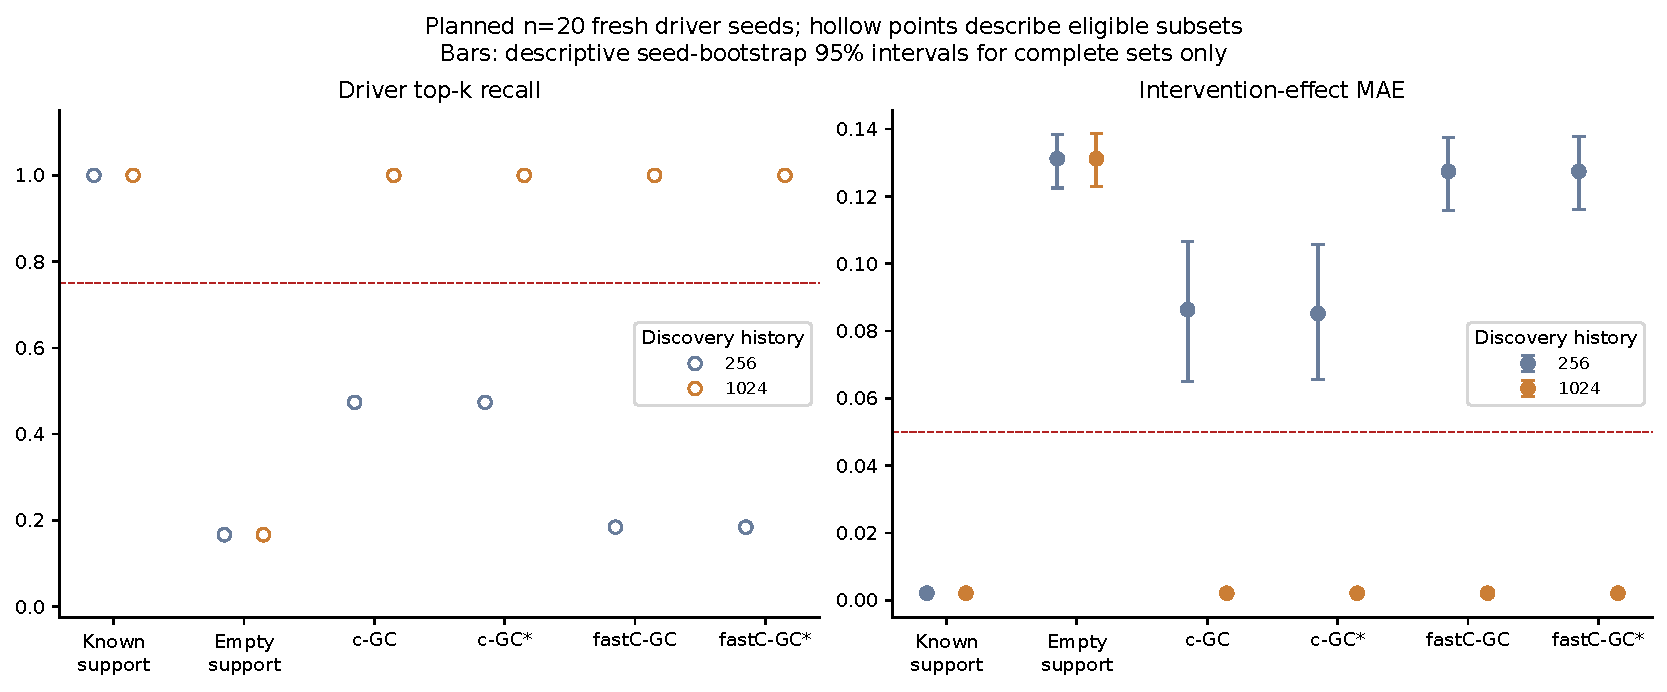
\includegraphics[width=\linewidth]{figures/01-fresh-seed-history.pdf}
\caption{Paired fresh-seed history comparison. Filled points and bars summarize
complete planned seed sets with descriptive seed-bootstrap 95\% intervals.
Hollow points show eligible-subset descriptions without an interval or a
complete-set acceptance claim. Dashed lines are the frozen ranking/MAE gates.}
\end{figure}\FloatBarrier

\section{Eligibility and the predeclared group intervention}
The following rows lack an intervention-positive individual neuron under the
0.10 simulator-effect threshold. They remain in the study. The group candidate
list was fixed before evaluation, including the pair of neurons 0/1; its recovery
is a descriptive diagnostic, not a new retrospective acceptance criterion.

\begin{table}[htbp]\centering\scriptsize\setlength{\tabcolsep}{3.5pt}
\caption{Directions ineligible for individual-neuron top-k under simulator truth.
The group column uses the strongest predeclared group. The final column counts
native methods nominating that group at their already frozen cutoffs.}
\begin{tabular}{@{}rrrrrrr@{}}\toprule
Seed & Source & Origins & Max neuron effect & Group truth & Native estimate range & Nominate\\\midrule
20012 & 1 & 6 & 0.021484 & 0.230469 & $[0.230469,\ 0.230469]$ & 4/4 \\
\bottomrule\end{tabular}\end{table}

A positive joint effect with individually subthreshold effects makes individual
ranking inapplicable; an estimated graph cannot change that simulator gold set.
The complete-set individual-ranking criterion therefore remains unmet when a
planned direction has no gold neuron, even if the known-support and native
readouts recover the joint intervention accurately. This is an eligibility and
causal-unit issue, rather than evidence that all native discovery failed.
Any future group-aware acceptance rule must be frozen on fresh seeds. Candidate
group discovery itself is not tested by providing the designed pairs here.

\section{Untouched null-test specificity}
One independent null seed contributes one event: any false nominee across the
candidates and supported directions. Table~\ref{tab:null} reports per-method
one-sided exact 95\% upper bounds \citep{clopper1934confidence}. Zero events in 60
seeds gives approximately 0.04870. Calibration and null validation are separate;
neither implies simultaneous coverage across methods or strong non-null FDR.

\begin{table}[htbp]\centering\small
\caption{Frozen operational cutoffs and complete null-test audit.}\label{tab:null}
\begin{tabular}{@{}lrrrr@{}}\toprule
Method & Cutoff & False-event seeds & Exact upper & Null gate\\\midrule
Known support & 0.100 & 0/60 & 0.048703 & pass \\
Empty support & 0.100 & 0/60 & 0.048703 & pass \\
c-GC & 0.100 & 0/60 & 0.048703 & pass \\
c-GC* & 0.100 & 0/60 & 0.048703 & pass \\
fastC-GC & 0.100 & 0/60 & 0.048703 & pass \\
fastC-GC* & 0.100 & 0/60 & 0.048703 & pass \\
\bottomrule\end{tabular}\end{table}

\begin{figure}[htbp]\centering
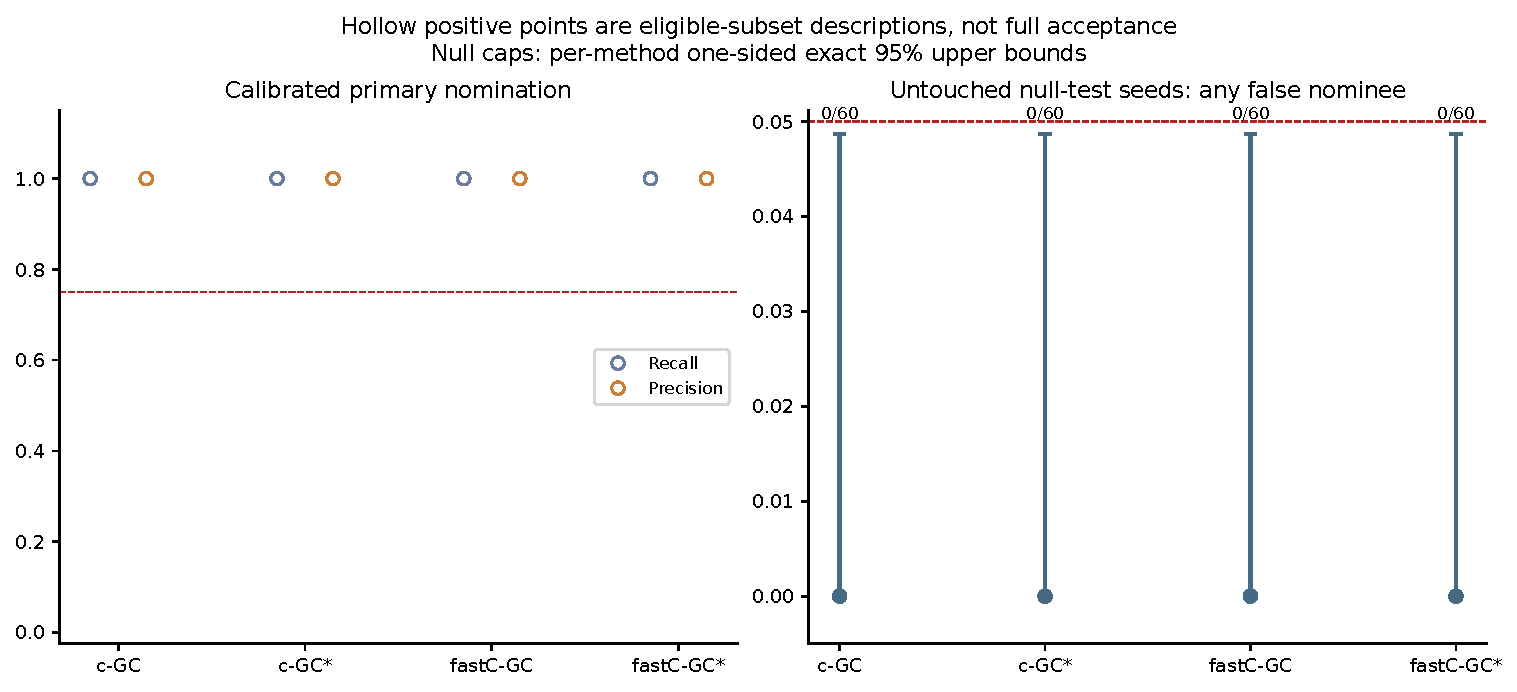
\includegraphics[width=\linewidth]{figures/02-nomination-and-null.pdf}
\caption{Positive nomination descriptions and untouched-null uncertainty.
Hollow positive points use eligible subsets; null caps are per-method one-sided
Clopper--Pearson 95\% upper bounds. Passing the null gate does not override failed
positive eligibility or establish biological specificity.}
\end{figure}\FloatBarrier

\section{Paired discovery-history effects}
Within each seed, histories share full mechanism-fitting data, evaluation origins,
oracle probabilities and rollout noise. Only discovery context changes. Table~\ref{tab:paired}
reports 1,024-minus-256 MAE changes; negative values favor the longer history.
Intervals resample independent seed differences 2,000 times \citep{efron1979bootstrap}.
The four native sign tests form one prespecified Holm family
\citep{holm1979sequential}. Their p-values concern sign tendency and cannot
override primary gates. The secondary history receives no calibrated null claim.

\begin{table}[htbp]\centering\small\setlength{\tabcolsep}{4pt}
\caption{Paired MAE changes, probability units. Controls receive no native-family
Holm p-value. Intervals are descriptive percentile-bootstrap 95\% intervals.}
\label{tab:paired}
\begin{tabular}{@{}lrrrr@{}}\toprule
Method & Paired seeds & Mean change & Descriptive 95\% interval & Holm p\\\midrule
Known support & 20 & 0.000000 & $[+0.000000,\ +0.000000]$ & -- \\
Empty support & 20 & 0.000000 & $[+0.000000,\ +0.000000]$ & -- \\
c-GC & 20 & -0.084267 & $[-0.104276,\ -0.063666]$ & 3.05e-05 \\
c-GC* & 20 & -0.083144 & $[-0.102957,\ -0.063170]$ & 3.05e-05 \\
fastC-GC & 20 & -0.125372 & $[-0.135274,\ -0.113743]$ & 7.63e-06 \\
fastC-GC* & 20 & -0.125372 & $[-0.135268,\ -0.113719]$ & 7.63e-06 \\
\bottomrule\end{tabular}\end{table}
\begin{figure}[htbp]\centering
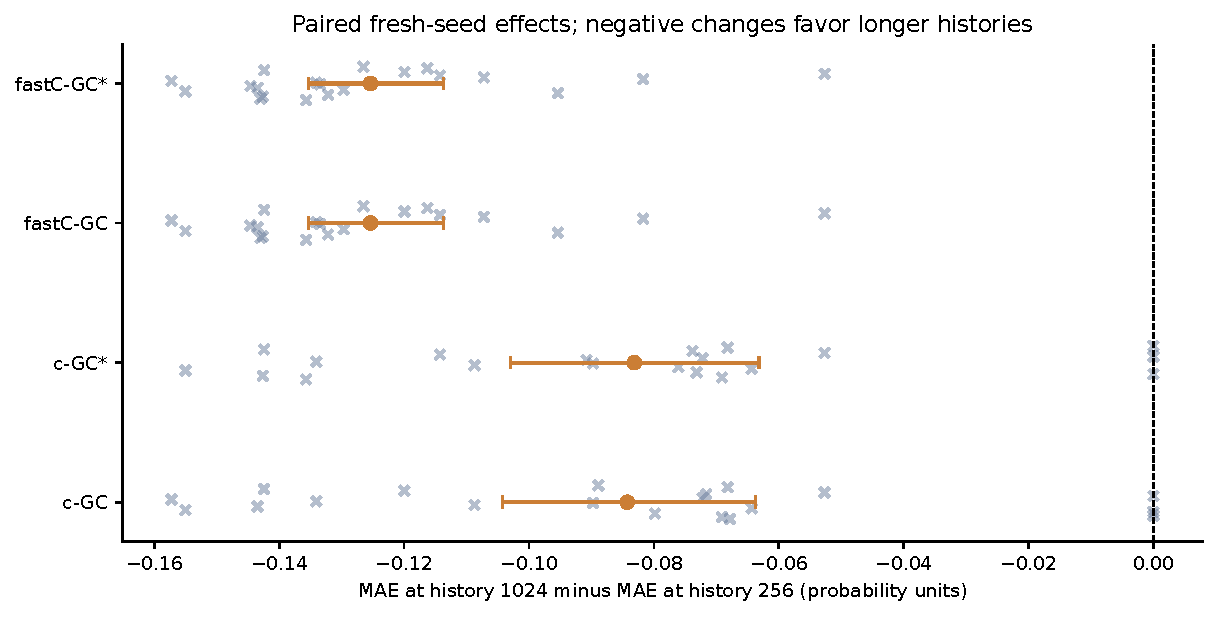
\includegraphics[width=\linewidth]{figures/03-paired-mae-changes.pdf}
\caption{Every native paired seed difference. Crosses are individual process-seed
changes; dots/bars are complete-set means and descriptive bootstrap 95\% intervals.}
\end{figure}\FloatBarrier

\section{Discussion and next decision}
The useful comparison is effect estimation against the known- and empty-support
controls across fresh seeds, together with a separate fixed-rule null audit.
Accurate effects and favorable conditional rankings can coexist with an unmet
complete-set ranking gate when individual effects are subthreshold but the joint
effect is positive. Reporting the latter as zero recovery would be incorrect; silently
dropping it to declare full acceptance would also change the frozen protocol.

The study changes the strength of evidence for the favorable mechanism control,
not the data-generating assumptions. Full observability, the matched nonlinear
basis, predeclared endpoint and designed candidate pairs remain limitations.
The previous latent/manifold benchmark remains a failed evaluation. Calibration
that retains the old 0.10 floor does not itself improve point estimates; its
contribution is a separate cutoff-selection procedure followed by untouched null
validation. No performance gain should be attributed to graph similarity, which
was not used. A future graph comparison can address representation and group
candidate generation, but cannot make an individual-neuron gold set exist in a
joint-only intervention case.

The frozen all-four acceptance flag remains \textbf{False}; the exact failed
gates and all individual seed values are preserved in the JSON and CSV evidence.
Prospective group-aware eligibility and robustness to observation/functional
misspecification are distinct next tests; repeated optimization on these inspected
test seeds would risk selection bias \citep{cawley2010overfitting}.

\section{Evidence and reproduction}
Study fingerprint: \path{12816838bd2fd250710b454e37b2a42e2fbc45dd789f6d0f91a56594ccedf101}. The parent directory contains the frozen
protocol, calibration evidence, full cell/native artifacts and implementation
snapshot. This report exports stored summaries without refitting or changing the
decision. See \path{seed-metrics.csv}, \path{statistics.json},
\path{eligibility-diagnostics.json}, \path{stats-appendix.md} and
\path{figure-catalog.md}. The implementation-test log records the regression suite;
the project protocol supplies the reference-verification audit.
{\small\setlength{\bibsep}{1pt}\bibliographystyle{plainnat}\bibliography{references}}
\end{document}
